\documentclass[10pt,a4paper]{ULBreport}
\usepackage[utf8]{inputenc}
\sceau{pic/official_logos/sceauULB.png}
\graphicspath{ {./pic/} }
\usepackage{multirow}
\usepackage{listings}
\usepackage{color} 
\usepackage{setspace} 
\usepackage{amsmath}
\usepackage{mathrsfs}
\usepackage{bm}
\usepackage[mathscr]{eucal}
\usepackage{hyperref}
\usepackage{pdfpages}
\usepackage{biblatex}
\usepackage{floatrow}
\usepackage{subcaption} 
\usepackage{siunitx}
\usepackage[many]{tcolorbox}
\usepackage{multirow}
\usepackage{listings}
\usepackage[dvipsnames]{xcolor}
\usepackage{fancyvrb}
\usepackage{graphicx}

\usepackage{xstring}
\usepackage{etoolbox}

% Colors



\begin{document} 


	\titleULB{
	title={V2V communication project},
    studies={M1-IRELE},
    course ={ELEC-H415 Communication Channels},
    author={\textit{Author :} \\ Colot Emmeran },
    date={\textbf{Academic year :} \\ 2024 - 2025},
    teacher={\textit{Professor : } \\ De Doncker Philippe},
    logo={pic/official_logos/logos.jpg},
    manyAuthor
	}

%\listoftables % ToC for tables

%\listoffigures % ToC for figures

\chapter*{Introduction}

In this project, a vehicle to vehicle (V2V) communication system is studied. The goal is to model the communication channel between two cars moving at the same speed. The road is straight and surrounded by buildings on which the signal can bounce. \\
The project is divided into two parts: the first one is a theoretical study of the channel and the second one presents the results of a simulation of this environment. The simulation is done using a raytracing algorithm that computes the paths of the rays between the two cars. Most of the experimental results are compared to the theoretical model and the differences are explained. \\

The parameters of the simulation are as follows:
\begin{itemize}
    \item Carrier frequency: $f_c = 5.9GHz$
    \item RF bandwidth: $B = 100MHz$
    \item Receiver sensitivity: $P_{RX, \text{min}} = -70dBm$
    \item Transmitter power: $P_{TX} = 0.1W$
    \item TX and RX antennas: vertical $\lambda/2$ dipoles
    \item Buildings relative permittivity: $\epsilon_r = 4$
    \item Number of bounces: $3$
    \item Distance between the two cars: $d \leq 1000m$
    \item Local areas length: $5m$
\end{itemize}




\chapter{Theoretical preliminaries}

\section{Equivalent electric circuit}

\begin{figure}[H]
    \centering
    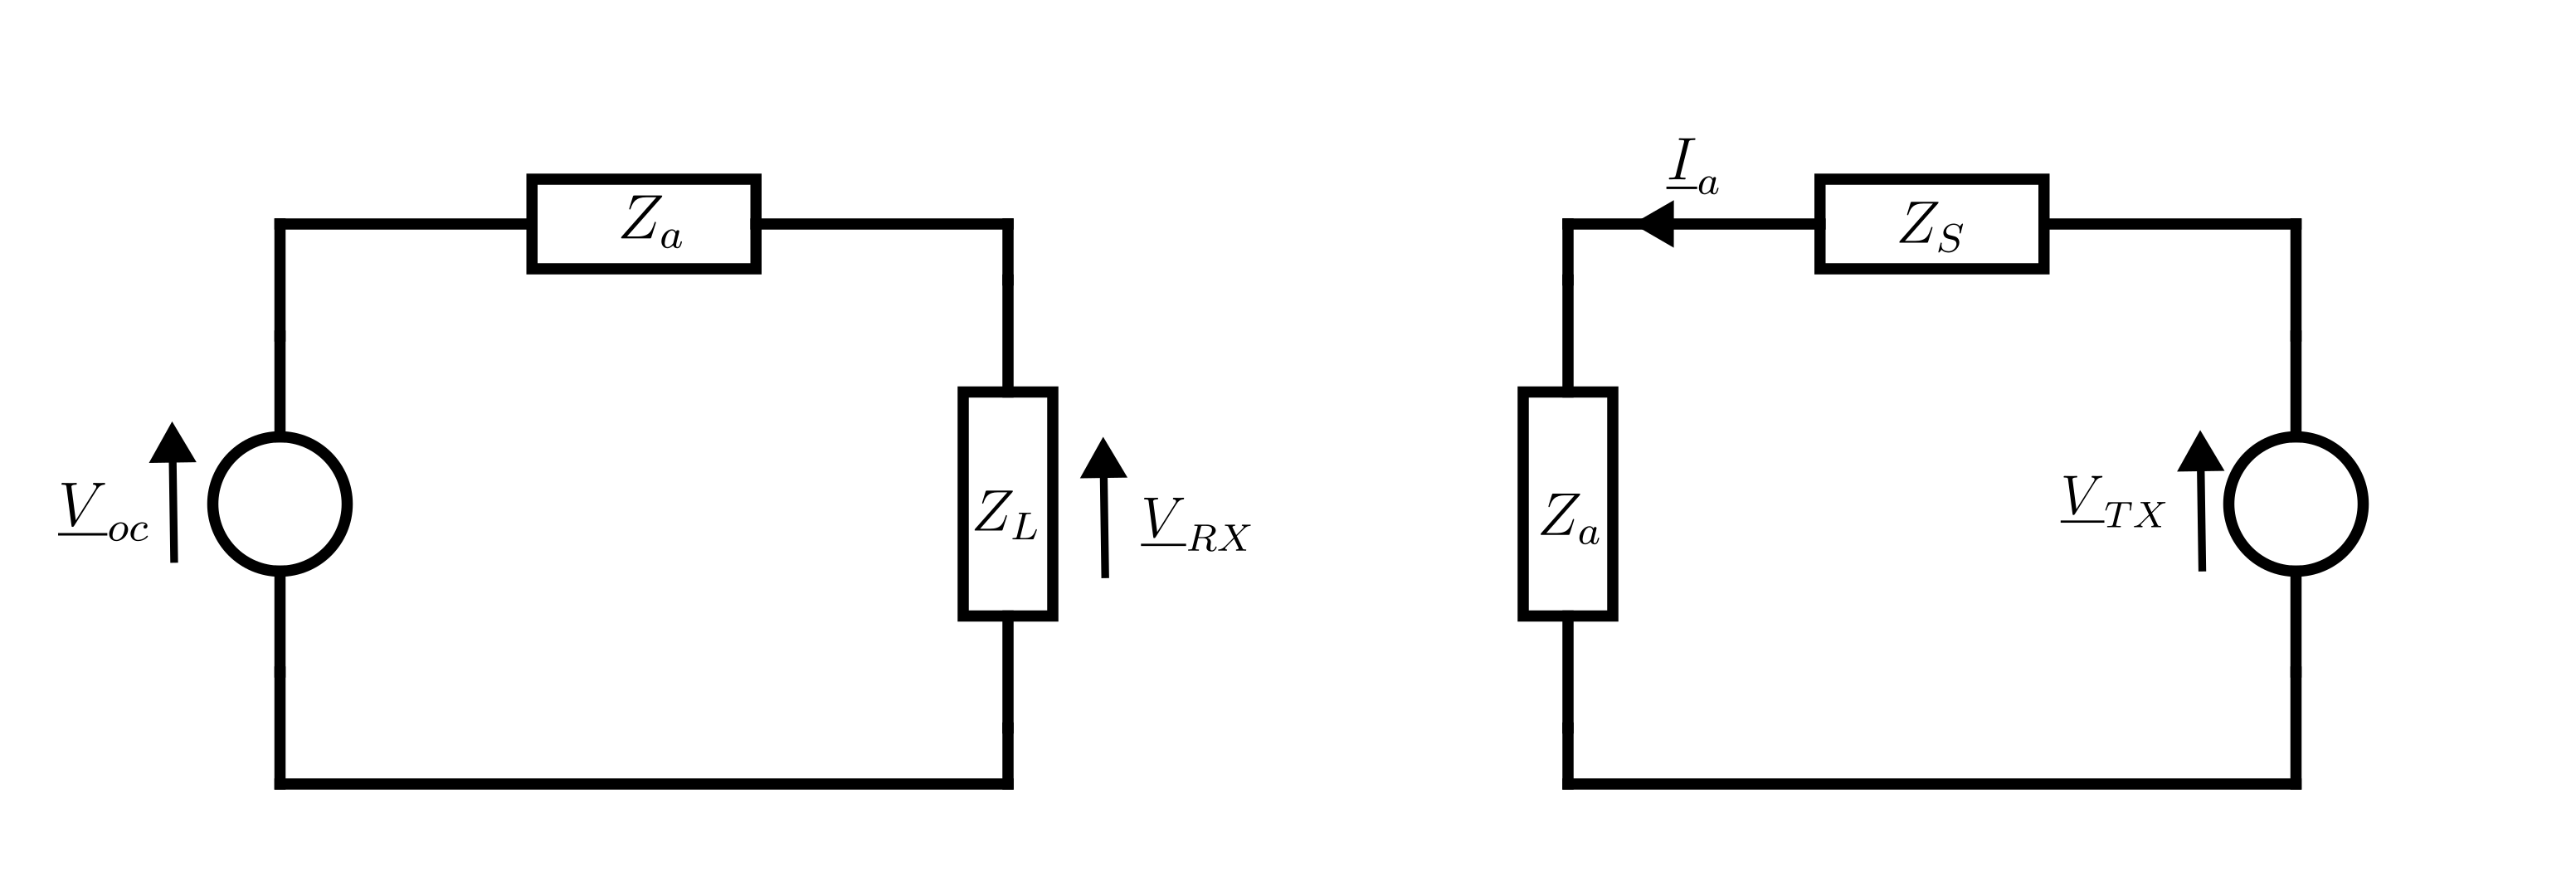
\includegraphics[width=1\textwidth]{circuit.png}
    \caption{Equivalent electric circuit of the RX antenna (left) and the TX antenna (right)}
    \label{fig:equivalent_electrical_circuit}
\end{figure}

Fig \ref{fig:equivalent_electrical_circuit} shows the equivalent electrical circuit at RX and TX where $\underline{V}_{oc}$ is the induced voltage, $\underline{V}_{\text{RX}}$ the voltage at the output of the RX antenna, $\underline{V}_{\text{TX}}$ the one at the input of the TX antenna and $\underline{I}_{a}$ the current entering the TX antenna.\\

\section{Equivalent height}

As both antennas are vertical $\lambda/2$ dipoles, their equivalent heights can be analytically computed:
\vspace{-1cm}

\begin{align*}
    \vec{h}_e (\theta, \phi) = \frac{\lambda}{\pi} \frac{\cos\left(\frac{1}{2}\cos \theta\right)}{\sin ^2 \theta}\vec{1_z}\\
    \vec{h}_{e\perp} (\theta, \phi) = -\frac{\lambda}{\pi} \frac{\cos\left(\frac{\pi}{2}\cos \theta\right)}{\sin \theta}\vec{1_\theta}
\end{align*}

Where $\theta$ and $\phi$ are respectively the polar and the azimuthal angles. This means that the horizontal plane (in which the rays in the simulation propagating) corresponds to $\theta = \pi/2$. The transverse equivalent height is then reduced to the following, where it does not depend on the azimuthal angle $\phi$:

\begin{align*}
    \vec{h}_{e\perp} (\phi) = -\frac{\lambda}{\pi} \vec{1_{\theta}}\\
\end{align*}

\section{Emitted electric field}

The transverse part of the equivalent height gives rise to an expression for the emitted electric field.
\vspace{-1cm}

\begin{align*}
    \underline{\vec{E}}(\vec{r}) &= -j\omega \underline{I}_a \frac{\mu_0}{4\pi}\frac{e^{-j\beta r}}{r}\vec{h}_{e\perp}(\theta, \phi) \\
    &= j\omega \underline{I}_a \frac{\mu_0\lambda}{4\pi^2}\frac{e^{-j\beta r}}{r} \vec{1_{\theta}} \\
    &= j \frac{\underline{I}_a \mu_0 c}{2\pi} \frac{e^{-j\beta r}}{r} \vec{1_{\theta}}\\
    &= j \frac{\underline{I}_a Z_0}{2\pi} \frac{e^{-j\beta r}}{r} \vec{1_{\theta}}
\end{align*}

To make the transmission parameters appear in the electric field expression, $\beta$ and $\underline{I}_a$ must be replaced with the formulas given below.
\vspace{-1cm}

\begin{align*}
    \beta &= \frac{2\pi f_c}{c}\\
    \underline{V}_{\text{TX}} &= (Z_a + Z_S) \underline{I}_a
\end{align*}

Wich yields

\begin{equation*}
    \underline{\vec{E}}(\vec{r}) = j \frac{\underline{V}_{\text{TX}}}{2\pi}\frac{Z_0}{Z_a + Z_S} \frac{e^{-\frac{j2\pi f_c r}{c}}}{r} \vec{1_{\theta}}
\end{equation*}

The last step is to replace the travel distance $r$ with $c \tau$ as the wave is propagating at the speed of light in free space. The electric field thus becomes:

\begin{equation*}
    \underline{\vec{E}}(\vec{r}) = j \frac{\underline{V}_{\text{TX}}}{2\pi}\frac{Z_0}{Z_a + Z_S} \frac{e^{-j2\pi f_c \tau}}{c\tau} \vec{1_{\theta}}
    \label{eq:emitted_electric_field}
\end{equation*}

\section{Received voltage}

The voltage at the output of the antenna $\underline{V}_{\text{RX}}$ can be deduced from the equivalent electric circuit \ref{fig:equivalent_electrical_circuit} as it is a simple voltage divider. Assuming matching impedances between the antenna and the load, we have:
\vspace{-1cm}

\begin{align*}
    \underline{V}_{\text{RX}} = \frac{Z_L}{Z_a + Z_L} \underline{V}_{oc} = \frac{1}{2} \underline{V}_{oc}\\
    \underline{V}_{oc} = -\left . \vec{h}_{e\perp}(\theta, \phi)\right\vert_{\theta = \pi/2} \cdot \underline{\vec{E}}_i
\end{align*}

Where $\underline{\vec{E}}_i$ is the incoming electric field which is equal to the radiated field in \ref{eq:emitted_electric_field}. It is here assumed that there was no reflexion, refraction or transmission through another material. This allows to find the votages at the receiver side as a function of the voltage at the transmitter side.
\vspace{-1cm}

\begin{align*}
    \underline{V}_{oc} &= \frac{\lambda}{\pi} \cdot \underline{E}_i\\
    &= j\frac{\lambda\underline{V}_{\text{TX}}}{2\pi^2}\frac{Z_0}{Z_a + Z_S}\frac{e^{-j 2\pi f_c \tau}}{c\tau}\\
    \underline{V}_{\text{RX}} &= j\frac{\lambda}{4\pi^2}\frac{Z_0}{Z_a + Z_S}\frac{e^{-j 2\pi f_c \tau}}{c\tau} \underline{V}_{\text{TX}}
\end{align*}

For later use, the time of flight $\tau$ is replaced by the traveled distance $d$, which is more convenient for the simulation. $Z_0$, $Z_a$, and $Z_S$ can also be replaced by $120\pi$, $\frac{720\pi}{32}$, and $\frac{720\pi}{32}$, respectively (assuming once again that the impedances are matched).\\

\begin{equation}
    \underline{V}_{\text{RX}} = j\frac{2 \lambda }{3\pi^2}\frac{e^{-j\frac{2\pi f_c d}{c}}}{d}\underline{V}_{\text{TX}}
    \label{eq:voltage_RX}
\end{equation}

\chapter{LOS channel}
\label{sec:LOS_channel}

\section{Impulse response}

Assuming the communication takes place via a LOS ray only, the channel impulse response $h(\tau)$ is defined as follows:

\begin{equation*}
    h(\tau) = \frac{\alpha_1 e^{-j\frac{2\pi f_cd_1}{c}}}{d_1} \delta\left(\tau - \tau_1\right)
\end{equation*}

\section{Transfer function}

Where $d_1$ is the distance of propagation and $\tau_1$ he propagation delay of the direct ray. $\alpha_1$ (which might be complex) takes into account a phase change or attenuation due for example to reflections whereas the imaginary exponential next to it corresponds to the phase change due to the propagation delay. \\
The transfer function $H(f)$ of the channel is found by taking the Fourier transform of $h(\tau)$
\vspace{-1cm}

\begin{align*}
    H(f) &= \int_{-\infty}^{\infty} h(\tau) e^{-j2\pi f \tau} d\tau\\
    &= \alpha_1\frac{e^{-j\frac{2\pi f_c d_1}{c}}}{d_1}e^{-j2\pi f \frac{d_1}{c}}\\
    &= \alpha_1\frac{e^{-j \frac{2\pi (f+f_c)d_1}{c}}}{d_1}\\
\end{align*}
\vspace{-2.5cm}

\section{Narrowband channel}

The narrowband impulse response of the channel $h_{\text{NB}}(\tau)$ is, in the case of a single ray, simply equal to $h(\tau$) where the impulse $\delta\left(\tau - \tau_1\right)$ has been removed. This is because the narrowband hypothesis states that the receiver perceives the sum of all rays instead of having each individual ray in separate taps. The signal received at the output of the channel $y(t)$ is given by:

\begin{equation*}
    y(t) = h_{\text{NB}}(t) x(t)
\end{equation*}
\begin{equation*}
    \text{where} \qquad h_{\text{NB}}(t) =\alpha_1\frac{e^{-j \frac{2\pi f_cd_1}{c}}}{d_1}
\end{equation*}

Where $x(t)$ is the transmitted signal. \\

\section{Power analysis}

The ratio between the received power $P_{\text{RX}}$ and the transmitted power $P_{\text{TX}}$ is found with:
\vspace{-1cm}

\begin{align}
    \frac{P_{\text{received}}}{P_{\text{transmitted}}} &= \frac{\left| h(\tau) \right|^2}{2} \nonumber\\
    &= \frac{\alpha_1^2}{d_1^2}
    \label{eq:power_approx}
\end{align}

This result can be compared with the Friis formula, given by:

\begin{equation}
    P_{\text{RX}}(d) = P_{\text{TX}} G_{\text{TX}}(\theta_{\text{TX}}, \phi_{\text{TX}})G_{\text{RX}}(\theta_{\text{RX}}, \phi_{\text{RX}})\left(\frac{\lambda}{4\pi d}\right)^2
    \label{eq:friis_formula}
\end{equation}

By comparing the two equations, the value of $\alpha_1$ can be deduced. It is equal to the product of the gains of the antennas $G_{\text{TX}}$ and $G_{\text{RX}}$ under and square root multiplied by the wavelength $\lambda$ divided by $4\pi$ and it is proven in a few lines here under:\smallskip\\
The power lost in the air during the propagation is proportional to the inverse of the distance squared. By comparing the Poynting vectors $\bm{\vec{\mathscr{S}}}_{\text{TX}}$ and $\bm{\vec{\mathscr{S}}}_{\text{RX}}$:

\begin{equation}
    \frac{\left|\bm{\vec{\mathscr{S}}}_{\text{RX}}\right|}{\left|\bm{\vec{\mathscr{S}}}_{\text{TX}}\right|} = \frac{1}{d_1^2}
    \label{eq:poynting}
\end{equation}

To compare the received and the injected power, the Poynting vectors should be replaced by the powers before and after transmission.
\vspace{-1cm}

\begin{align*}
    \left|\bm{\vec{\mathscr{S}}}_{\text{TX}}\right| = G_{\text{TX}} P_{\text{TX}}\\
    \left|\bm{\vec{\mathscr{S}}}_{\text{RX}}\right| A_{eRX} = P_{\text{RX}}\\
    \text{where} \quad \quad A_{eRX} = G_{\text{RX}}\left(\frac{\lambda}{4\pi}\right)^2
\end{align*}

When placed back in eq \ref{eq:poynting}, the expression can be put next to \ref{eq:power_approx} which gives:
\vspace{-1cm}

\begin{align*}
    \frac{P_{\text{RX}}}{P_{\text{TX}}} = \frac{G_{\text{TX}} A_{eRX}}{d_1^2} &= \frac{\alpha_1^2}{d_1^2}\\
    \frac{G_{\text{TX}} G_{\text{RX}}}{d_1^2} \left(\frac{\lambda}{4\pi}\right)^2 &= \frac{\alpha_1^2}{d_1^2}\\
    \alpha_1 &= \sqrt{G_{\text{TX}} G_{\text{RX}}} \frac{\lambda}{4\pi}
\end{align*}

Now that the Friis formula has been proved to be equivalent to the theoretically proved model, \ref{eq:friis_formula} can be used. It is simplified as the antennas are considered to be lossless dipoles. The gains are therefore replaced by $\frac{16}{3\pi}$, the theoretical gain of vertical half-wave dipoles in the horizontal plane.

\begin{equation}
    \frac{P_{\text{RX}}}{P_{\text{TX}}} = \frac{16}{9\pi^2} \left(\frac{\lambda}{\pi d_1}\right)^2
    \label{eq:power_friis_simplified}
\end{equation}

Two deductions can be made of this result: 
\begin{itemize}
    \item The power loss on the channel depends on the square of the distance between the emitter and the receiver. It implies that doubling the range of an antenna would need a multiplication of the transmitting power by a factor 4.
    \item A more surprising result is the wavelength squared appearing at the numerator. It shows that there is always a compromise between data rate and power consumption as a larger wavelength will indeed be less attenuated but the maximal data rate will then be lowered because of the decreased transmission frequency.
\end{itemize}

\section{About the moving cars}
The emitter and receiver are cars that are moving at the same speed. This is not taken into account anywhere later as the impact is minimal. To measure this, the coherence time of the channel is used. This parameter is defined as the time during which the channel can be considered as constant and it is given by:
\begin{equation*}
    \Delta t_c = \frac{1}{2}\frac{\lambda}{v}
\end{equation*}
Where $v$ is the speed of the cars. Taking for it the maximal speed of a car in Belgium (120km/h) as it will give the lowest coherence time, it gives:
\begin{equation*}
    \Delta t_c = 762.7\mu s
\end{equation*}
Because the bandwidth of the channel is 100 MHz, more than 64 ksymbols can be sent in this time. With a modern modulation such as 64-QAM, this allows to send packets of more than 350 kbits. This size should be used as maximum size for the packets in order for the channel to be considered as constant during the transmission. \\







\chapter{Full channel, narrowband analysis}
\section{Raytracing}

After having implemented a raytracing algorithm, the simulation is able to compute every path from the transmitter to the receiver. Figure \ref{fig:raytracingDemo} shows the result of the simulation for a 20m wide road surrounded by buildings. 

\begin{figure}[H]
    \centering
    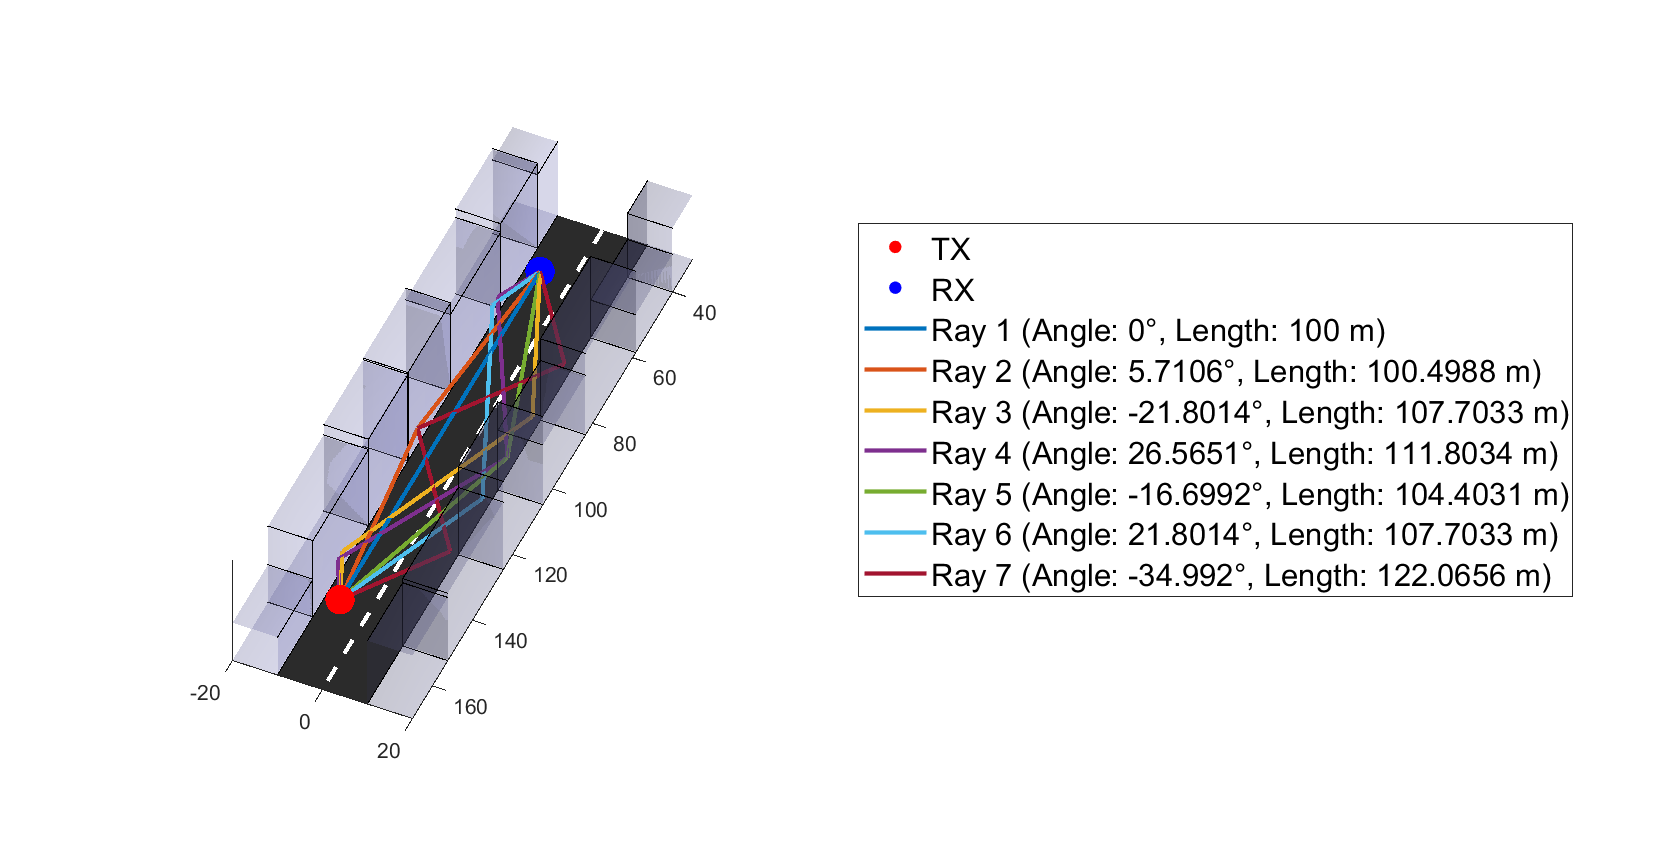
\includegraphics[width=1\textwidth]{3_1.eps}
    \caption{Simulation of the raytracing algorithm. The number of bounces is limited to 3 and the two communicating cars are spaced by 100m. The angles are computed between the ray and the road direction.}
    \label{fig:raytracingDemo}
\end{figure}

\section{Received voltage}
The received voltage has been computed on the same setup using equation \ref{eq:voltage_RX} to which the reflection coefficients $\Gamma_{\perp}$ have been added. 

\begin{align*}
    \Gamma_{\perp} = \frac{\cos \theta_i - \sqrt{\epsilon_r-\sin^2\theta_i}}{\cos \theta_i + \sqrt{\epsilon_r-\sin^2\theta_i}}
\end{align*}

The voltage carried by each ray is shown in figure \ref{fig:voltageDemo} using a colormap and the exact values are given in table \ref{tab:ray_properties}. The total received voltage is found with:
\vspace{-1cm}

\begin{align*}
    \left|V_{\text{tot}}\right| &= \left|\sum_{n=1}^{N} V_i\right|\\
    &= 419.5 \mu V
\end{align*}
\vspace{-1cm}

Where $N$ is the number of rays and $V_i$ the voltage carried by the $i^{th}$ ray. The total received voltage is not equal to the sum of the voltages because of the different phase of each ray. \\

\begin{table}[H]
    \centering
    \begin{tabular}{|c|c c c|}
        \hline
        Ray Index & Ray physical angle (°) & Ray length (m) & Carried voltage ($\mu V$)\\ \hline
        1 & 90.0 & 100.0 & 258.3\\ \hline
        2 & 78.7 & 102.0 & 202.0\\ \hline
        3 & -68.2 & 107.7 & 102.4\\ \hline
        4 & 59.0 & 116.6 & 38.2\\ \hline
        5 & -78.7 & 102.0 & 202.0\\ \hline
        6 & 68.2 & 107.7 & 102.4\\ \hline
        7 & -59.0 & 116.6 & 38.2\\ \hline
    \end{tabular}
    \caption{Properties of each ray shown in figure \ref{fig:raytracingDemo}. For the voltage computation, the physical angle is now the one between the ray and the normal to the wall. The carried voltage has been added.}
    \label{tab:ray_properties}
\end{table}

\begin{figure}
    \centering
    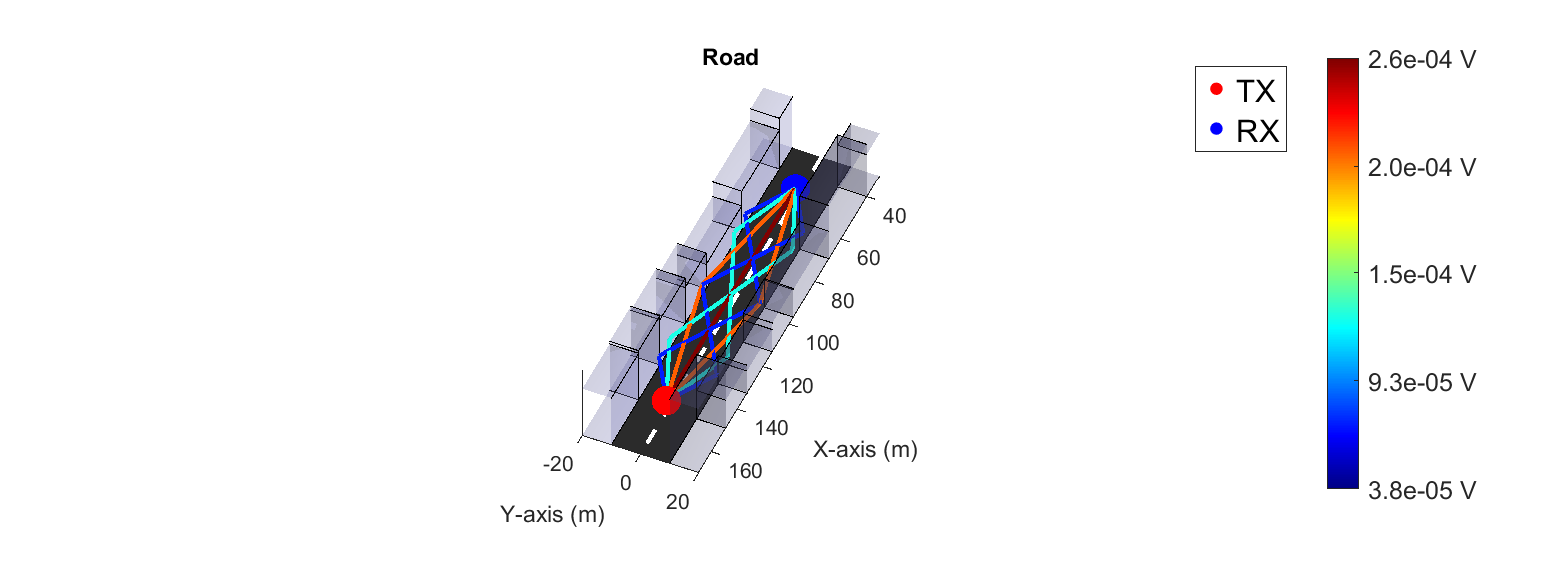
\includegraphics[width=0.8\textwidth]{3_2.eps}
    \caption{Received voltage for each ray}
    \label{fig:voltageDemo}
\end{figure}

Figure \ref{fig:voltageDemo} and table \ref{tab:ray_properties} clearly show that the power is decreasing as the length of the ray increases. This means that the LOS ray is the one carrying the most power. From a certain distance, the length of every MPC will start to be closer to the one of the ray that does not bounce and their contribution will then be as important as the one of the LOS ray. This will be detailed with the Rice factor in section \ref{sec:fading}.

\section{Received power}
\label{sec:power_analysis}
By varying the distance between the two communicating cars between 0 and 1000m, a comparison is made between the raytracing simulation and the theoretical model on figure \ref{fig:P_RX(d)}. The simulated power is computed by taking the square of $V_{OC}$ divided by $Z_L \mathbin{\|} Z_a$ (see figure \ref{fig:equivalent_electrical_circuit}) and the theoretical power is computed using equation \ref{eq:power_friis_simplified} (Friis formula).

\begin{figure}[H]
    \centering
    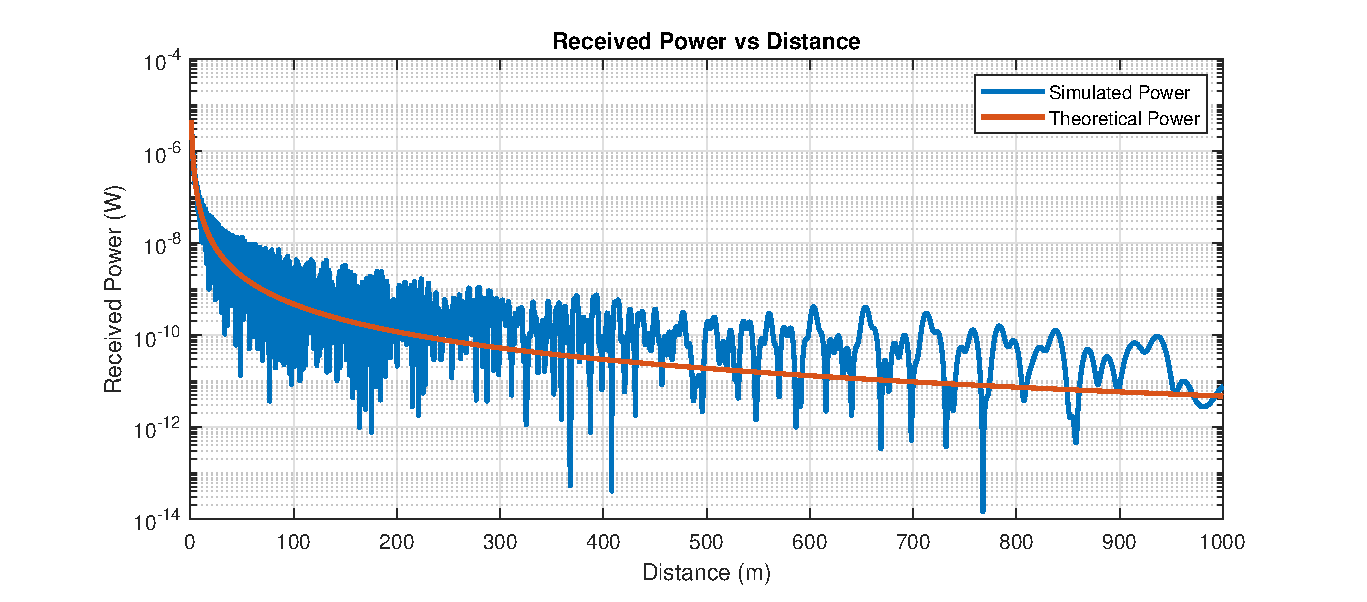
\includegraphics[width=1\textwidth]{3_3.eps}
    \caption{Received power as a function of the distance between the two cars}
    \label{fig:P_RX(d)}
\end{figure}

For short distances, the LOS ray is the only one contributing to the received power which explains the good match of the simulation with theory. \\
After a few meters, the multi path components (MPC) start to have an impact on the received power and the resulting interferences make the simulated power $<P_{RX}>$ oscillate around the theoretical power $\ll P_{RX} \gg$. This effect is called shadowing and it will be modeled later on.\\

\section{Rice factor}
\label{sec:fading}
The oscillation around the expected power can be modeled with a Rice distribution as the LOS ray is the strongest one. The Rice factor $K$ is defined as the ratio between the power of the LOS ray and the power of the other rays:

\begin{align*}
    K = \frac{a_0^2}{\sum_{n=1}^{N}a_n^2}
\end{align*}

where $a_n$ is the amplitude of the $n^{th}$ ray with $a_0$ the amplitude of the LOS ray. As those amplitudes vary with distance, figure \ref{fig:K(d)} shows the rice factor as a function of the distance between the two cars. 

\begin{figure}[H]
    \centering
    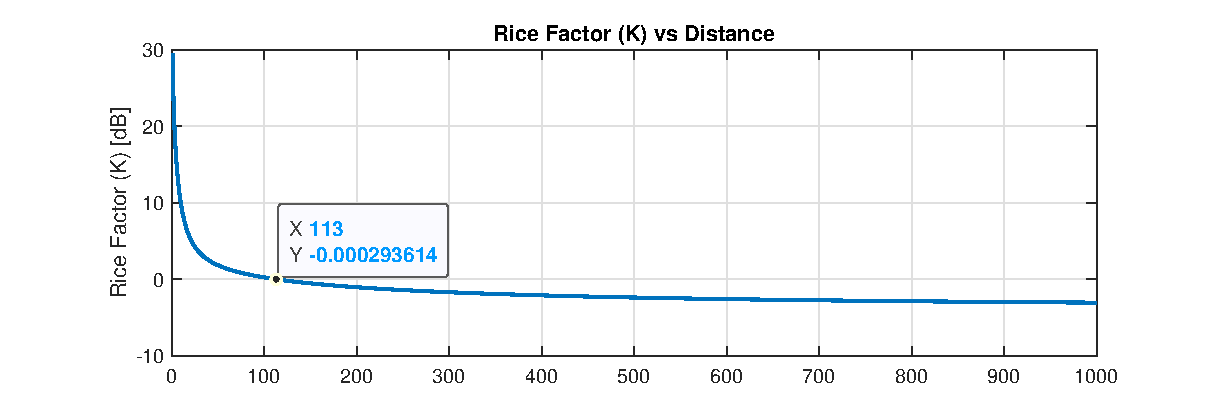
\includegraphics[width=1\textwidth]{3_4.eps}
    \caption{Rice factor as a function of the distance between the two cars. The highlighted point is the distance from which the LOS ray is not the strongest one anymore.}
    \label{fig:K(d)}
\end{figure}

The Rice factor is a good indicator of the portion of the power that is due to the LOS ray. The point at which it becomes smaller than 1 (or 0dB) is the point at which the power due to the LOS ray is equal to the sum of the power of the other rays. \\
The Rice factor close to the emitter is high, which indicates that the fading is low and $K$ becomes smaller after only a few meters. As seen in figure \ref{fig:P_RX(d)}, the received power oscillates more around the expected value because the MPC's start to generate fading.\\

\section{Average received power in local areas}
The average received power in local areas is computed using:
\vspace{-1cm}

\begin{align}
    <P_{\text{RX}}> &= \frac{1}{8 Z_a} \sum_{n=1}^{N} \left| V_{\text{OC,n}} \right|^2\\
    &= \frac{1}{45\pi} \sum_{n=1}^{N} \left| V_{\text{RX,n}} \right|^2
    \label{eq:average_power}
\end{align}
\vspace{-1cm}

Where the sum is done over all the received rays. Figure \ref{fig:average_power} shows the average received power in local areas with a width of 5m. The power is in dBm as it quicly becomes very small. \\
To have enough data points to model the whole area, the transmitter is placed at all the possible positions (spaced by $1m$) on the width of the road. The receiver is then placed on every tile of $5x5m$ and the average power is computed using equation \ref{eq:average_power}. Figure \ref{fig:average_power} then shows this average power that is again averaged on every position of the emitter\footnote{The impact of placing the emitter on multiple points instead of just placing it in the center of the road has close to no impact on the path loss model. It has still been done as the model is now suited for any transmitter position on the road}.

\begin{figure}[H]
    \centering
    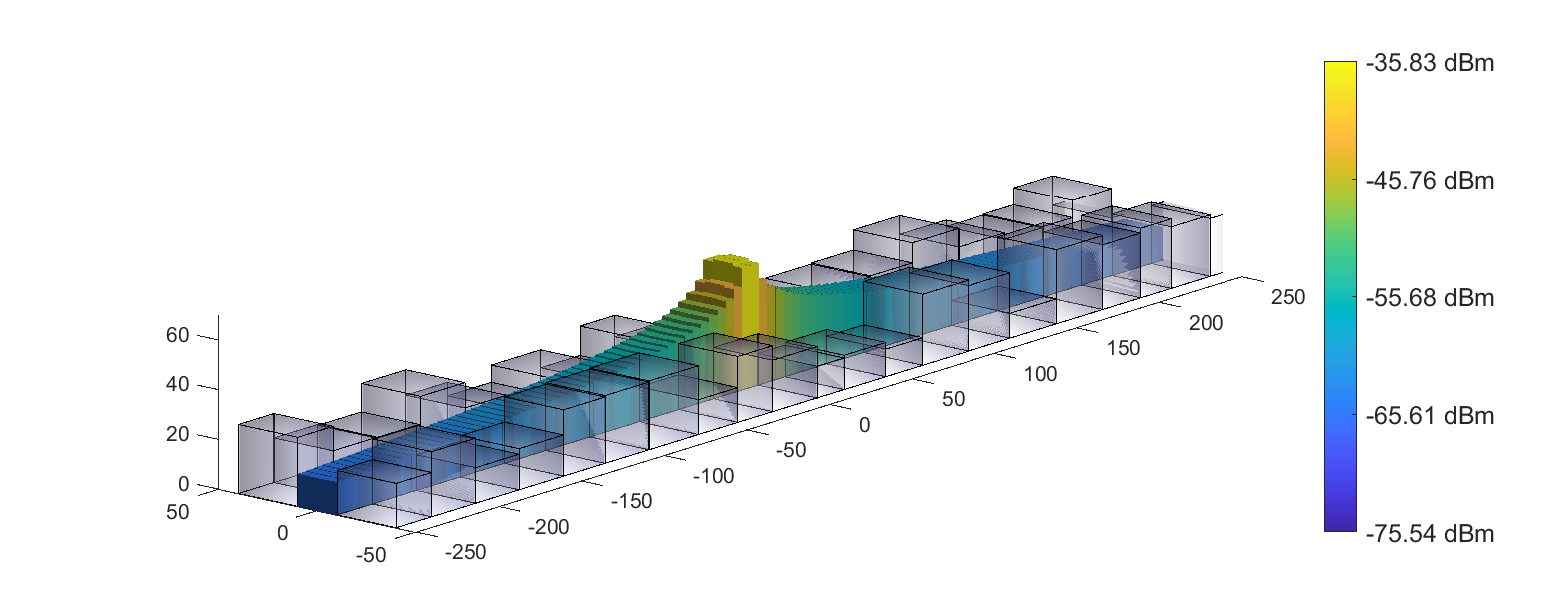
\includegraphics[width=1\textwidth]{3_5.eps}
    \caption{Average received power in local areas of 5m}
    \label{fig:average_power}
\end{figure}

For visualization purposes, figure \ref{fig:average_power} is limited to 250m. The colormap indicates that the power obtained at the edge of the plot is approximately equal to $-60$ dBm. This is still $10$ dBm above the receiver sensitivity the cell radius will certainly by larger than 250m. It will be computed in section \ref{sec:cell_range} with the path loss model that has to be established.\\

The path loss of the channel $L(d)$ and the path loss that does not depend on the antennas $L_0(d)$ are defined (with every term in dB) as:


\begin{subequations}
    \label{eq:path_loss}
    \begin{align}
        L(d) &= P_{\text{TX}} - P_{\text{RX}}\\
        L_0(d) &= L(d) + G_{\text{TX}} + G_{\text{RX}}
    \end{align}
\end{subequations}

The canonical model for $L_0(d)$ is:

\begin{align*}
    L_0(d) = L_0(d_0) + 10 n \log_{10} \left(\frac{d}{d_0}\right)
\end{align*}

In which the parameters $L_0$ and $n$ must be found to fit the values of the simulation. $d_0$ has been arbitrarily set to 1m. The result is shown in figure \ref{fig:path_loss} and the resulting parameters give as path loss model:

\begin{align}
    \label{eq:path_loss_model}
    L_0(d) = 51.03 + 16.3 \cdot log_{10} \left(\frac{d}{1\text{m}}\right)
    \qquad
    \text{implying} \qquad \left\{
    \begin{array}{l}
        n = 1.63 \\
        L_0(d_0) = 51.03
    \end{array}
    \right.
\end{align}

\begin{figure}[H]
    \centering
    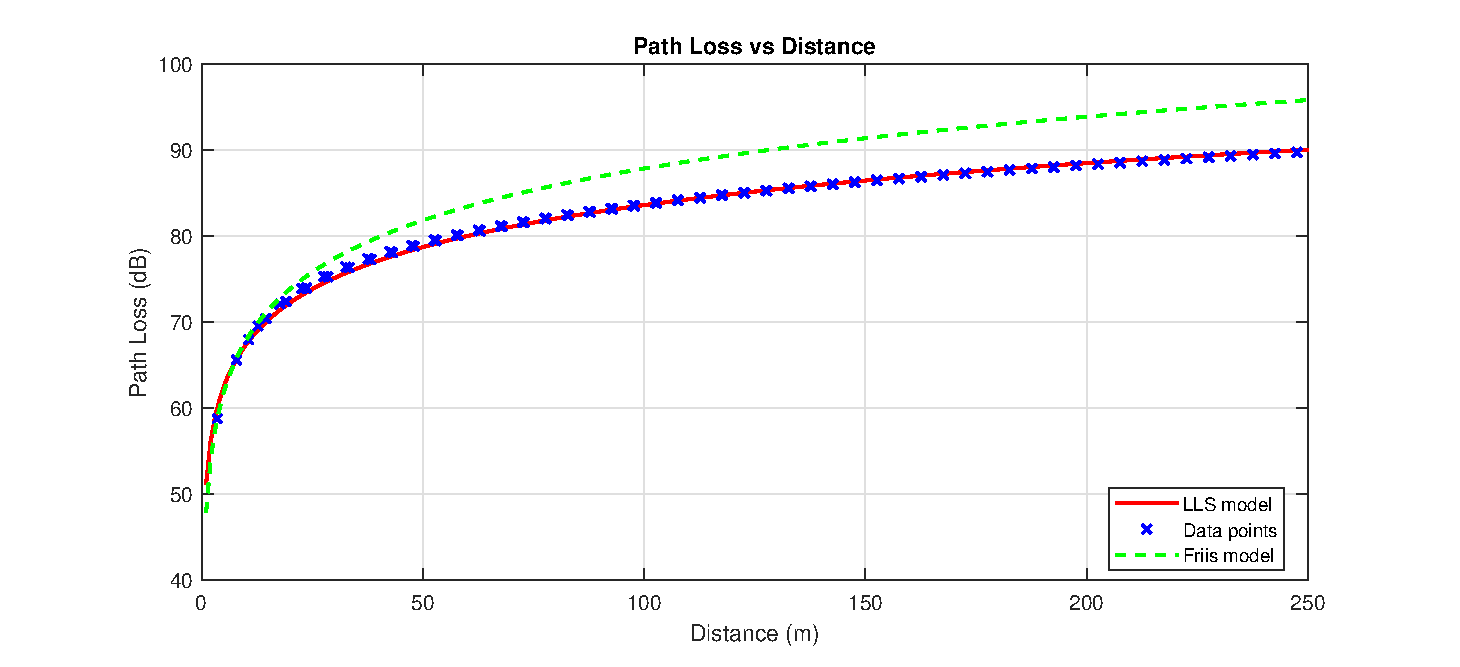
\includegraphics[width=1\textwidth]{3_5_model.eps}
    \caption{Path loss of the channel and fitted model, limited to 250m for visualization purposes}
    \label{fig:path_loss}
\end{figure}

\section{Model variability}

As the LLS estimator only gives a "\textit{best fit}" to the data, there is still a parameter to define: the variability $\sigma_L$. It is the standard deviation of the path loss around the fitted model defined in \ref{eq:path_loss_model} and its value here is:

\begin{equation*}
    \sigma_L = 0.225 \quad \text{dB}
\end{equation*}

The measured path loss is smaller than the one given by the Friis formula. This is because the simulation computes multiple rays that will (in the area averaging operation \ref{eq:average_power}) add up to a larger power than in a single ray model. The path loss model is therefore indeed supposed to be smaller than the Friis formula. \\

\section{Cell range}
\label{sec:cell_range}
The communication reliability can be found under the assumption that the power variations due to shadowing is log-normal distributed. In that case, the probability of a successful communication is given by:

\begin{equation}
    \label{eq:path_loss_probability}
    P_{\text{success}} = \frac{1}{2} \text{erfc}\left(\frac{M}{\sigma_L\sqrt{2}}\right) 
\end{equation}

Where $M$ is the fade margin, defined as the difference between the received power and the minimum power needed to decode the signal. The fade margins required for a certain communication reliability are given in table \ref{tab:fade_margins}. They have been found by plotting the error probability as a function of the fade margin (see figure \ref{fig:fade_margin}). \\
The cell range can also be computed for each value of $P_{\text{success}}$ using equation \ref{eq:path_loss} and \ref{eq:path_loss_model}. 

\begin{align*}
    L(d) &= P_{\text{TX}} - P_{\text{RX}}\\
    L_0(d_\text{max}) &= P_{\text{TX}} - P_{RX, \text{min}} + G_{\text{TX}} + G_{\text{RX}}\\
    51.0 + 16.3 \cdot log_{10} \left(\frac{d_{\text{max}}}{1\text{m}}\right) &= P_{\text{TX}} - P_{RX, \text{min}} + G_{\text{TX}} + G_{\text{RX}}
\end{align*}

The minimal received power $P_{RX, \text{min}}$ is the receiver sensitivity to which the fade margin is added. Putting the values of the left parameters in the equation gives:

\begin{align*}
    51.0 + 16.3 \cdot log_{10} \left(\frac{d_{\text{max}}}{1\text{m}}\right) &= 20 - (-70 + M) + 2 \times 10 \log_{10} \left(\frac{16}{3\pi}\right)\\
    \log_{10} \left(\frac{d_{\text{max}}}{1\text{m}}\right) &= \frac{43.6 - M}{16.3}\\
    d_{\text{max}} &= 10^{\frac{43.4 - M}{16.2}} \left[\text{m}\right]
\end{align*}

\begin{table}[H]
    \centering
    \begin{tabular}{|c c c|}
        \hline
        Communication reliability & Fade margin (dB) & Cell radius (m) \\ \hline
        50\% & 0 & 476.7 \\ \hline
        95\% & 0.371 & 452.3 \\ \hline
        99\% & 0.524 & 442.7 \\ \hline
    \end{tabular}
    \caption{Fade margins and cell radius for different communication reliability}
    \label{tab:fade_margins}
\end{table}

Because the error between the data and the fitted model is small (as proved both in figure \ref{fig:path_loss} and by the small value of $\sigma_L$), the cell radius varies very little with the communication reliability. 

\begin{figure}[H]
    \centering
    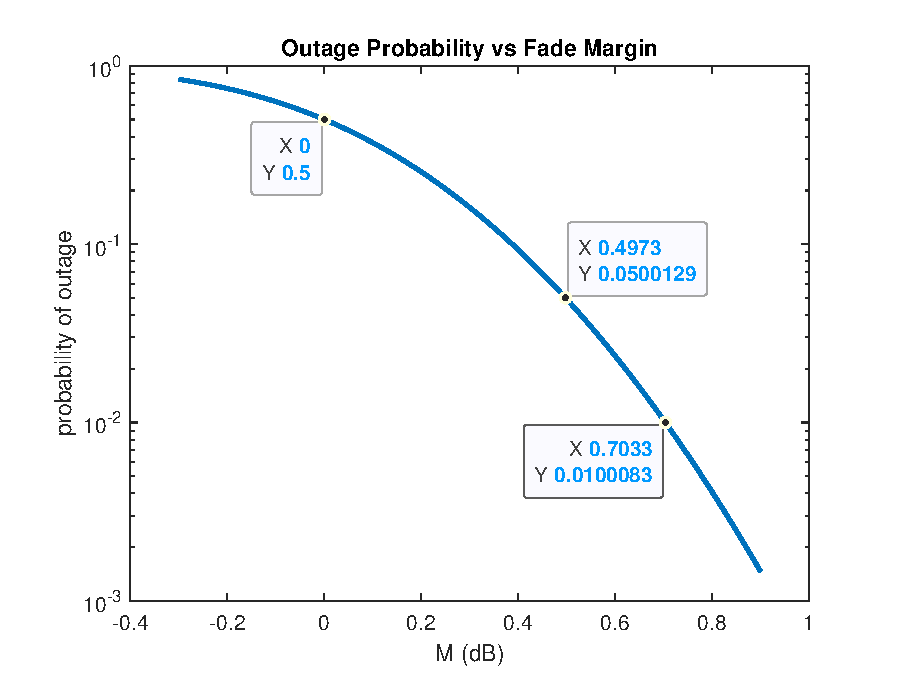
\includegraphics[width=1\textwidth]{3_7.eps}
    \caption{Fade margin as a function of the communication reliability, plotted using equation \ref{eq:path_loss_probability}}
    \label{fig:fade_margin}
\end{figure}





\chapter{LOS channel, wideband analysis}
\label{sec:LOS_channel_wideband}

\section{Impulse response and transfer function}
For the wideband model and if there is only a single ray, the impulse response of the channel is given by:

\begin{equation*}
    h(t) = \frac{e^{-j \frac{2\pi f_cd_1}{c}}}{d_1} \delta(t - \tau_1)
\end{equation*}

The impulse response and the corresponding transfer function (computed by taking the DFT of $h(t)$) are shown in figure \ref{fig:impulse_response} and \ref{fig:transfer_function}. 

\begin{figure}[H]
    \centering
    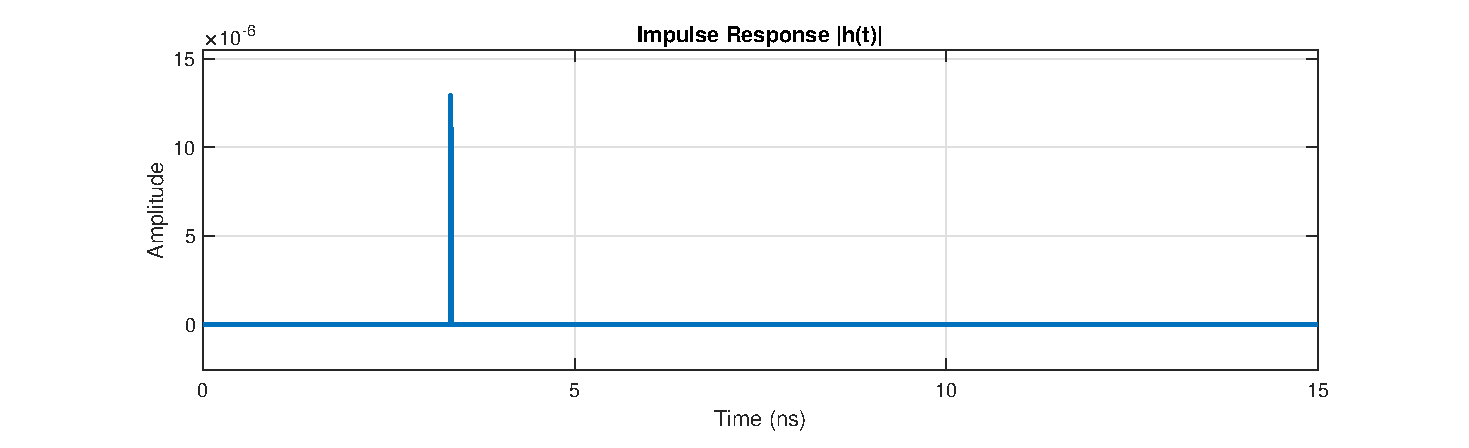
\includegraphics[width=1\textwidth]{4_1_temp.eps}
    \caption{Impulse response of the wideband channel with the LOS ray only for a transmitter and receiver separated by 1km} 
    \label{fig:impulse_response}
\end{figure}

\begin{figure}[H]
    \centering
    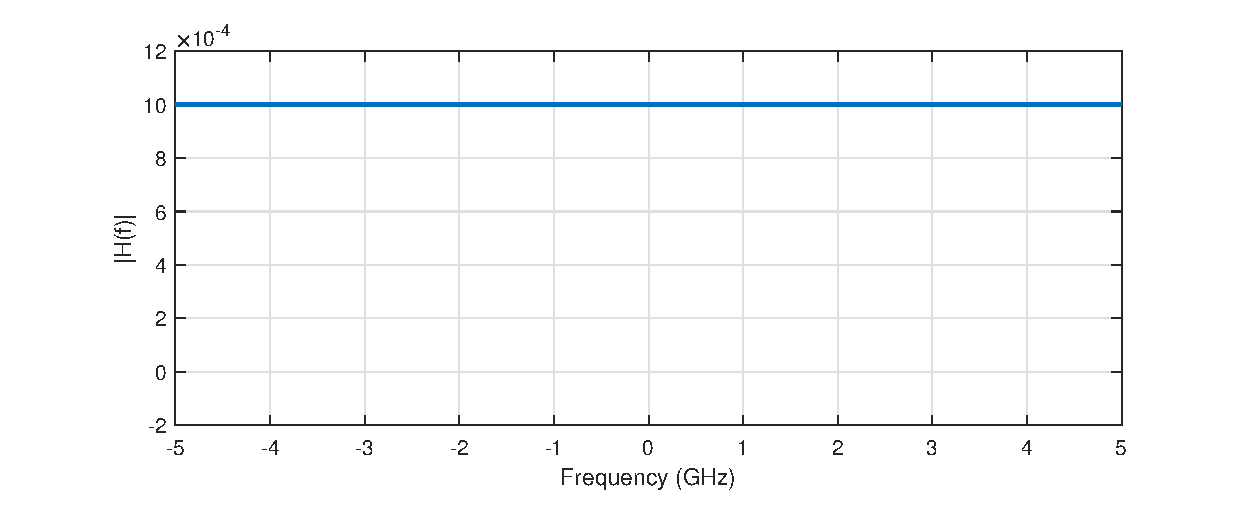
\includegraphics[width=1\textwidth]{4_1_freq.eps}
    \caption{Transfer function of the wideband channel with the LOS ray only for a transmitter and receiver separated by 1km}
    \label{fig:transfer_function}
\end{figure}

The impulse response is a single peak at a time corresponding to the time of flight of the LOS ray. The transfer function has a constant value over the frequency spectrum. This means that there is no frequency selectivity for a single ray, a result easily understandable as no frequency is less attenuated than another in free space. This is of course valid only because some assumptions have been made: there is no multipath propagation and no parasitic effects (gaseous absorption, rain attenuation, tropospheric scintillation, etc.).\smallskip\\

\section{Tapped delay line model}
Because of the limited bandwidth of the channel, the tapped delay line model is used to compute $h_{\text{TDL}}(t)$. The previous impulse response did not take into the fact that the receiver is only able to sample at the time resolution of the system $\Delta\tau = \frac{1}{B}$, where B is its bandwidth. The TDL model is found by:

\begin{equation}
    h_{\text{TDL}}(t) = \sum_{l=0}^{L} h_l(t) \delta(t - l\Delta\tau)
    \label{eq:h_TDL}
\end{equation}
\begin{equation*}
    \text{where} \qquad h_l(t) = \sum_{n=1}^{N} \alpha_n(t) \text{sinc}\left(B(\tau_n - l\Delta\tau)\right)
\end{equation*}

In those equations, $L$ is the maximal index of the temporal taps (linked with the maximal allowed delay) and $N$ is the number of rays, which is simply $1$ when only the direct ray is taken into account. $\alpha_1$ is different from the one defined in section \ref{sec:LOS_channel}, as it here takes the spacial dispersion into account:

\begin{equation*}
    \alpha_n = \frac{e^{\frac{-j2\pi f_c d_n}{c}}}{d_n} \cdot \prod_{b=1}^{B} \Gamma_{\perp, b} \qquad \text{where } B \text{ is the number of bounces of the } n^{th} \text{ ray}
\end{equation*}

What was presented above is the exact model of the TDL. A usual approximation is to say that the receiver simply sums up the rays that are arriving in the same time bin. This means that $h_l(t)$ is now equal to:
\begin{equation}
    h_l(t) = \sum_{\tau_n \in [l\Delta\tau, (l+1)\Delta\tau]} \alpha_n(t) 
    \label{eq:h_l}
\end{equation}

This approximation heavily simplifies the computation of $h_{\text{TDL}}(t)$ and it shows that each tap of \ref{eq:h_TDL} is uncorrelated with the others. This is known as the \textit{uncorrelated scattering}(US) assumption of the channel in the delay model. \\
The impulse response of the TDL model, under the US assumption, is then given by:

\begin{equation*}
    h_l(t) = \left\{
    \begin{array}{l}
        \alpha_1 \qquad \text{if } l\Delta\tau \leq \tau_1 < (l+1)\Delta\tau\\
        0 \qquad \text{otherwise}
    \end{array}
    \right.
\end{equation*}

The tapped delay line impulse response $h_{\text{TDL}}(t)$ is shown on figure \ref{fig:h_TDL_LOS}. It can be compared to $h(t)$ (in figure \ref{fig:impulse_response}) and the difference is that the peak has been moved to a tap (from 3.3334ns to 3.33ns)

\begin{figure}
    \centering
    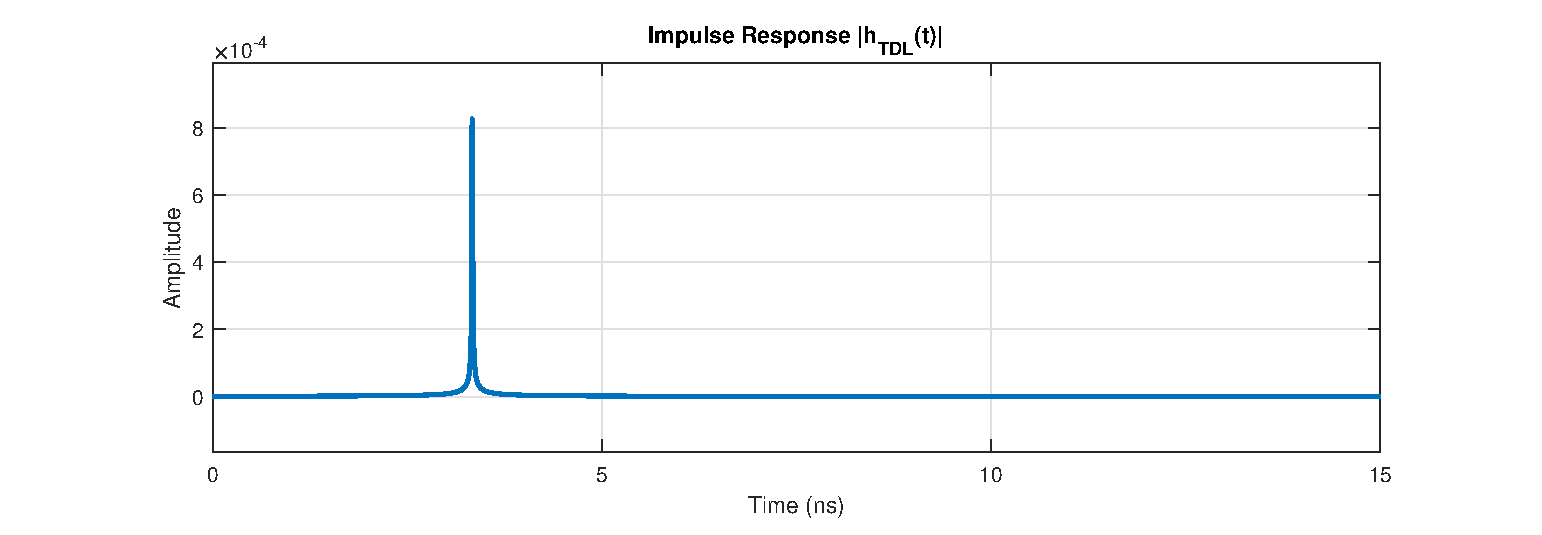
\includegraphics[width=1\textwidth]{4_2.eps}
    \caption{TDL impulse response of the wideband channel with the LOS ray only for a transmitter and receiver separated by 1km}
    \label{fig:h_TDL_LOS}
\end{figure}

\chapter{Full channel, wideband model}
\section{Impulse response}
This section do the same analysis as the previous one but for multiple rays. The impulse response is shown in figure \ref{fig:impulse_response_full}. \\

\begin{figure}[H]
    \centering
    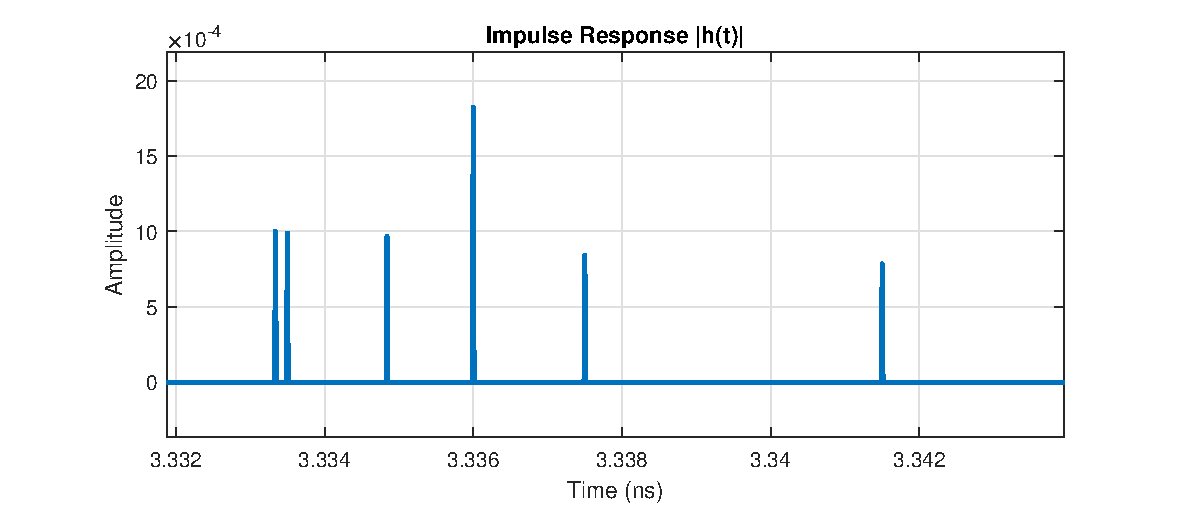
\includegraphics[width=1\textwidth]{5_1.eps}
    \caption{Impulse response of the wideband channel with multiple rays for a transmitter and receiver separated by 500m}
    \label{fig:impulse_response_full}
\end{figure}

The impulse response plot is zoomed in so the different peaks are visible. Because of the multiple peaks, interference will occur between the rays, causing some frequencies to be more attenuated than others during their propagation through the channel. This is the reason why the transfer function will not be constant anymore. \\

\section{Transfer function}

The transfer function plot is also only partially shown in order to focus around the carrier frequency $f_c = 5.9$GHz. This analysis shows that this choice for $f_c$ is not optimal as the amplitude of $H(f)$ is low around this frequency. A wiser choice would have been to choose a frequency around $f_c = 5.95$GHz, which has more than twice the amplitude, resulting in needing four times less power to transmit. This is of course only true for the simulated environment (so for a distance of 500m between the transmitter and receiver) and it makes the choice for an optimal carrier frequency difficult. \\

\begin{figure}[H]
    \centering
    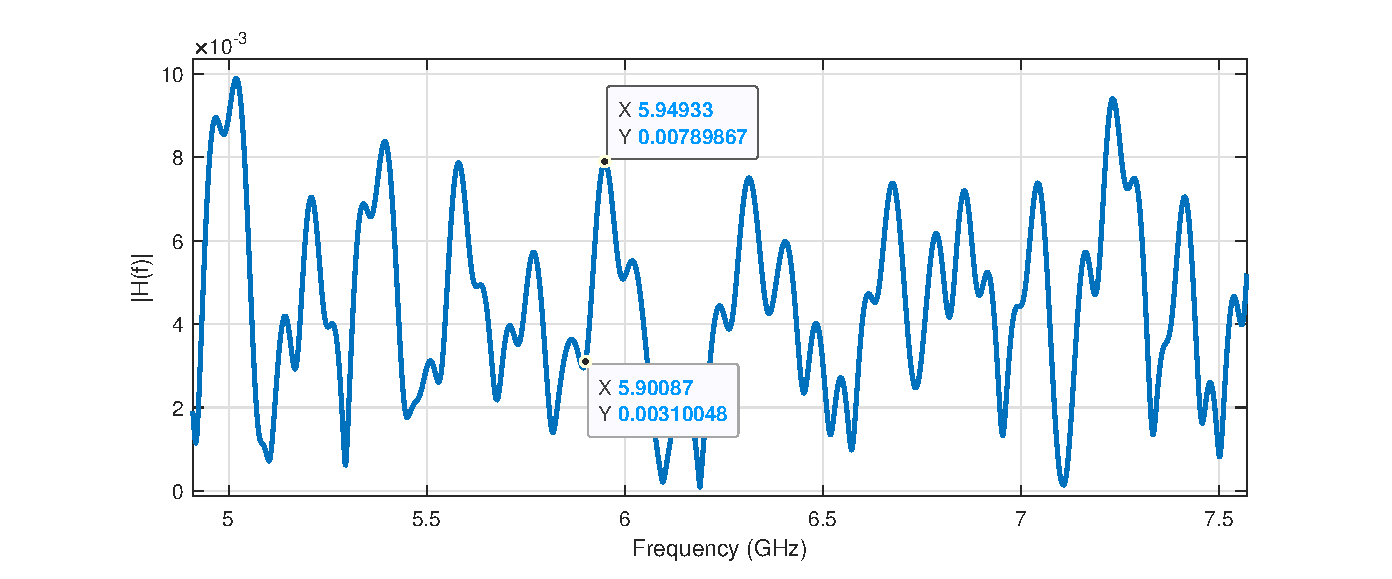
\includegraphics[width=1\textwidth]{5_2.eps}
    \caption{Transfer function of the wideband channel with multiple rays for a transmitter and receiver separated by 500m}
    \label{fig:transfer_function_full}
\end{figure}

\section{Tapped delay line model}

The impulse response of the tapped delay line model is computed using the same method as in section \ref{sec:LOS_channel_wideband}. First, $h_l(t)$ is computed using equation \ref{eq:h_l} and then the TDL impulse response is computed using equation \ref{eq:h_TDL}. The result is shown in figure \ref{fig:impulse_response_TDL}. The difference with the previous impulse response is that some peaks now arrive in the same time bin. This means that the receiver will not be able to distinguish between them and they will interfere with each other. 

\begin{figure}
    \centering
    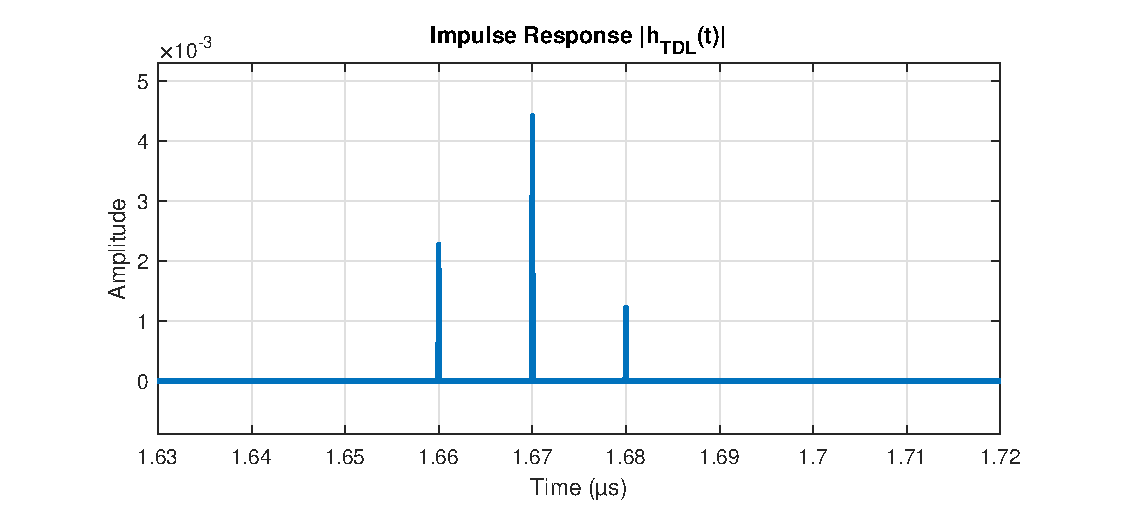
\includegraphics[width=1\textwidth]{5_3.eps}
    \caption{Impulse response of the TDL model with multiple rays for a transmitter and receiver separated by 500m}
    \label{fig:impulse_response_TDL}
\end{figure}



\chapter{Further analysis}
\section{Power Delay Profile}
\subsection{Description}
The power delay profile (PDP or $P(\tau)$) is defined as the expected power of the channel in every bin in the wideband model. As there is an expected value in its mathematical definition (see \ref{eq:pdp}), $h_l$ must be computed using equation \ref{eq:h_l} for a lot of different realizations of the channel. This has been done by placing the receiver at every possible position on the road (spaced by $5m$, as for the average power).

\begin{equation}
    P(\tau) = \sum_{l=0}^{L}\mathbb{E}\left[\left|h_{l}\right|^2\right] \delta(\tau - l\Delta\tau)
    \label{eq:pdp}
\end{equation}

\subsection{PDP result}

The PDP is shown in figure \ref{fig:pdp} and has been computed using equation \ref{eq:pdp}. It is limited to $1\mu s$ to have a better view of the peaks. It allows already to see a trend of the power to decrease with the bin index. This is due to the fact that the rays that are arriving later are traveling longer distances and are therefore more attenuated.\\

\begin{figure}[H]
    \centering
    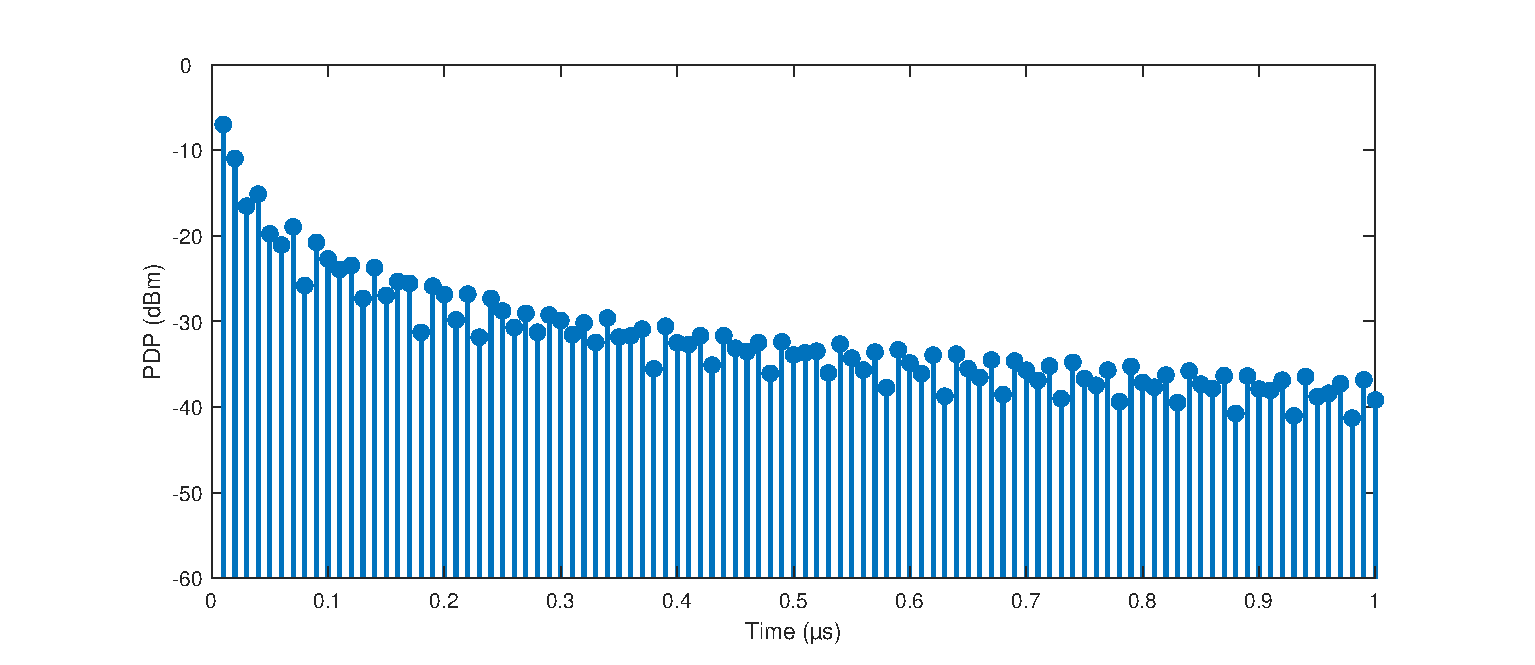
\includegraphics[width=1\textwidth]{6_0.eps}
    \caption{Power delay profile of the channel with at most 3 bounces}
    \label{fig:pdp}
\end{figure}

A few parameters can be extracted from the PDP. The first one is the total power $P$ which is defined as:

\vspace{-0.8cm}
\begin{align*}
    P &= \int_{0}^{+\infty} P(\tau) d\tau\\
    &= -3.41 \text{dBm}
\end{align*}
\vspace{-1cm}

The total power allows to compute the mean delay $\tau_m$:

\vspace{-0.8cm}
\begin{align*}
    \tau_m &= \frac{1}{P} \int_{0}^{+\infty} \tau P(\tau)  d\tau\\
    &= 0.11 \mu s
\end{align*}
\vspace{-1cm}

The mean delay is the time at which the power of the channel is maximal. It is short as the power at low delays is very high (let's not forget that \ref{fig:pdp} is in dBm).\\
The last parameter is the delay spread $\sigma_{\tau}$, which is defined as follows:

\vspace{-0.8cm}
\begin{align*}
    \sigma_{\tau} &= \sqrt{\frac{1}{P} \int_{0}^{+\infty} \tau^2 P(\tau) d\tau - \tau_m^2}\\
    &= 0.31 \mu s
\end{align*}
\vspace{-1cm}

This parameter is a measure of the dispersion of the rays. The larger it is, the more the rays are spread in time and the more difficult it will be to decode the signal. This is because the receiver will not be able to distinguish between two rays that arrive at different times but are close enough to be in the same time bin. \\
The relatively low delay spread in this case is due to the fact that each ray follows a path that is close to the one of the other rays. As their traveling distance is similar, they arrive at the receiver at a similar time and the delay spread is small. \\

\section{Different geometry}

\subsection{Description}

This section will analyze what happens when cars on perpendicular roads try to communicate with each other. The transmission cofficient of the rays that pass through buildings is supposed to be close to zero. Because of this, a lot of rays are removed and there is a need for a higher number of bounces. \\
\subsection{Power analysis}
The power analysis is done the same way as in section \ref{sec:power_analysis} but with a different setup. The 3D plot \ref{fig:3D_2} shows the average power received in local areas of 5m. with the transmitting car placed at 25m from the intersection center.

\begin{figure}
    \centering
    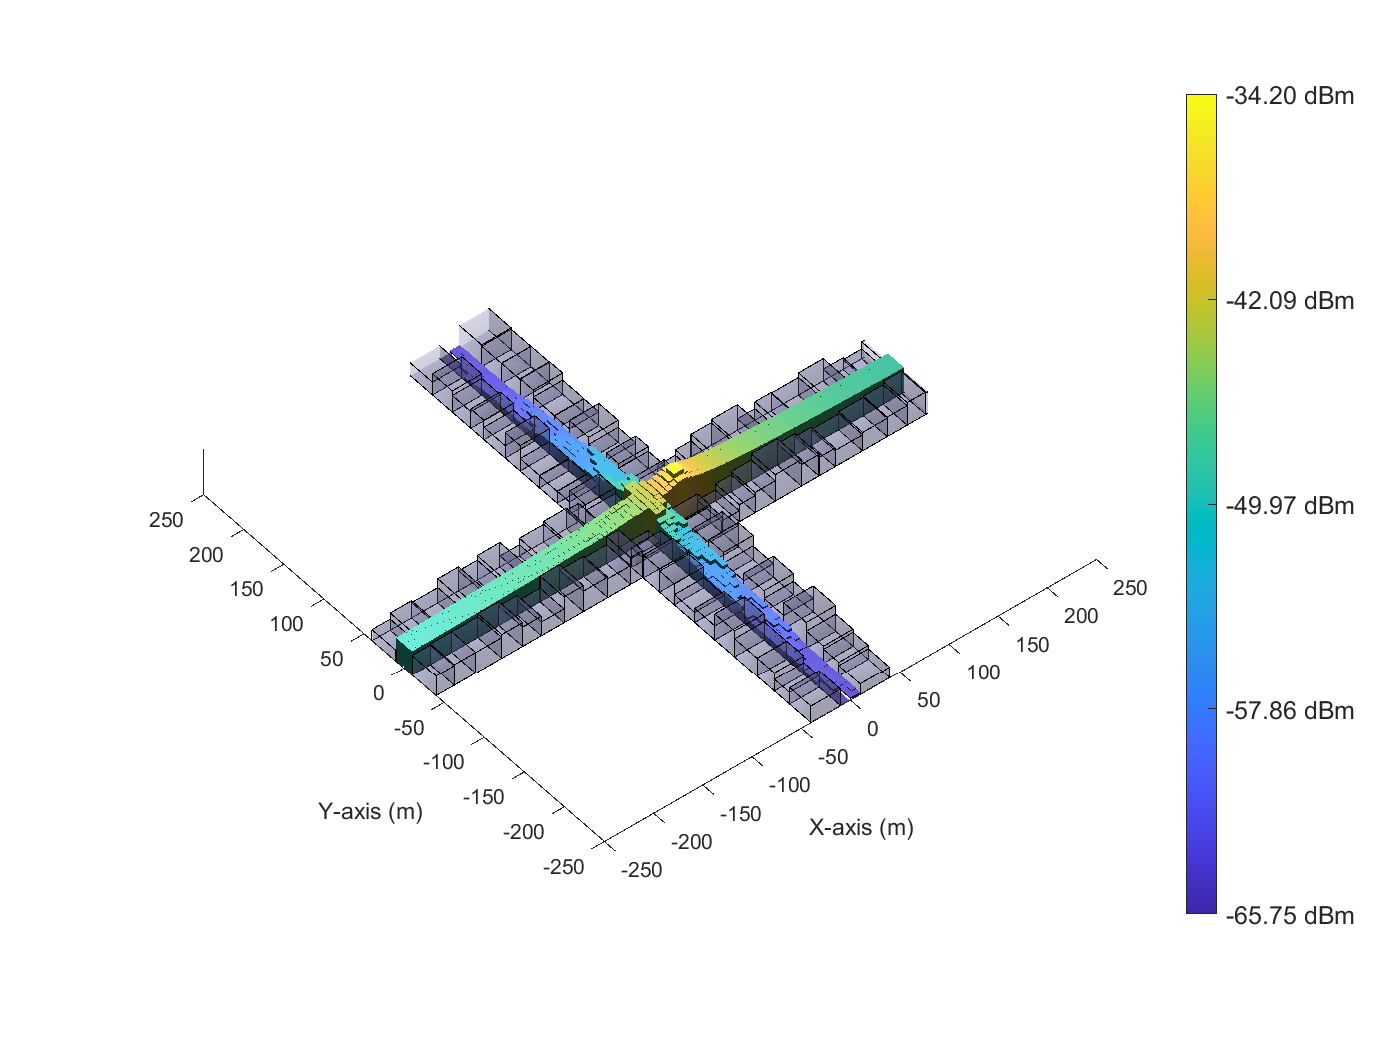
\includegraphics[width=1\textwidth]{6_1.eps}
    \caption{Average received power in local areas of 5m for a car placed at 25m from the intersection center with maximum 6 bounces}
    \label{fig:3D_2}
\end{figure}


As one can see, the power is now much less homogeneous than in the previous case and it becomes even more obvious when trying to model it. This was done the same way as previously and the fitted model together with the data points are shown in figure \ref{fig:path_loss_2}. The model is:
\vspace{-1cm}

\begin{align*}
    L_0(d) = 39.5 + 28.1 \cdot log_{10} \left(\frac{d}{1\text{m}}\right)\qquad
    &\text{implying} \qquad \left\{
    \begin{array}{l}
        n = 2.81 \\
        L_0(d_0) = 39.5
    \end{array}
    \right.\\
    \text{with } \qquad \sigma_L &= 12.8 \quad \text{dB}
\end{align*}

The data points in figure \ref{fig:path_loss_2} can be split in two groups: the points with a lower path loss, that stay close to the Friis model, and the points with a higher path loss. The first group corresponds to the positions on the same road as the transmitter and the values are quiet close to the ones in figure \ref{fig:path_loss}. \\
The second group corresponds to the cars on the perpendicular road. Those have a much higher path loss as a lot of rays are absorbed by the buildings. The fitted model being minimizing the least square error for the whole dataset, it is unable to properly fit to the data points. This is easily measured by the standard deviation which is now 40 times higher than the one computed for a single straight road. \\
Comparing those two groups with the Friis model, it can be seen that the perpendicular is worse because of the absorbed rays and the points on the same road are better because the MPC's allow to have a larger power than in open space. \\

\begin{figure}
    \centering
    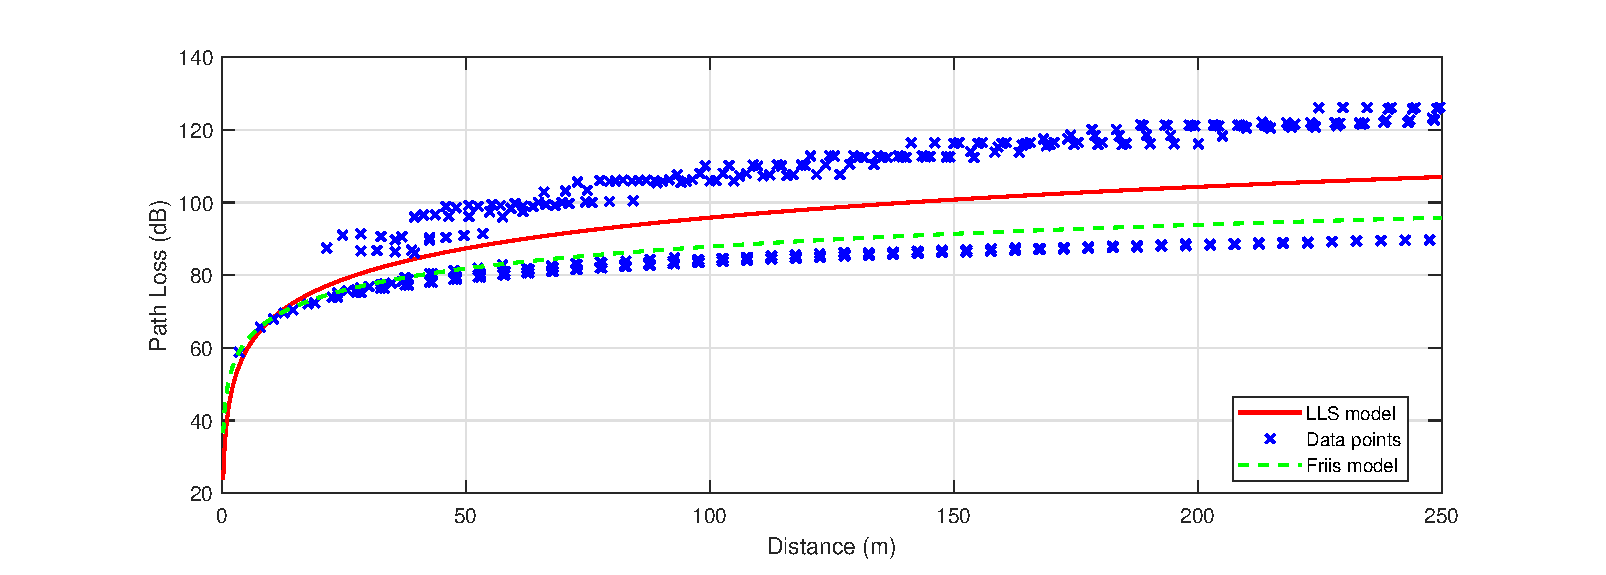
\includegraphics[width=1\textwidth]{6_2.eps}
    \caption{Path loss of the channel and fitted model for a car placed at 25m from the intersection center with maximum 6 bounces}
    \label{fig:path_loss_2}
\end{figure}

\subsection{Communication reliability}

The change in the model implies that the cell radius must be recomputed. A table with the fade margins and the cell radius is shown below. Because the variability is much higher, the range of the cell radius is rapidly decreasing when the required communication reliability increases. \\

\begin{table}[H]
    \centering
    \begin{tabular}{|c c c|}
        \hline
        Communication reliability & Fade margin (dB) & Cell radius (m) \\ \hline
        50\% & 0 & 90.4 \\ \hline
        95\% & 21.0 & 16.2 \\ \hline
        99\% & 29.7 & 7.9 \\ \hline
    \end{tabular}
    \caption{Fade margins and cell radius for different communication reliability}
    \label{tab:fade_margins_2}
\end{table}

Note that in such a case, the cell radius is not a good indicator of the range of the car. One can indeed see that a 99\% communication reliability is only possible for a car placed at less than 10m from the emitter but at such distances, there cannot be a wall between the two cars and the situation is identical to the one in section \ref{sec:power_analysis}. \\
A more realistic number is the one for 50\% communication reliability. The computed distance of 90m shows that the intersection has indeed a negative effect on the range. There is division by a factor $5$ of the cell radius, which corresponds to the need for 25 times more power at the emitter antenna to achieve the same range, as proved by \ref{eq:power_friis_simplified} in the first chapter. \\

%\printglossary

%\printglossary[type=\acronymtype]

%Bibliography
%\nocite{*}
%\printbibliography[type=article,title=Articles]

\end{document}	
